\documentclass[modern]{aastex61}

% \submitjournal{the Astrophysical Journal}

\usepackage{bm}

\newcommand{\todo}[1]{ \textcolor{red}{#1}}

\newcommand{\normal}[2]{{\cal N} \left( #1, #2 \right)}

\newcommand{\veclambda}{{\bm \lambda}}
\newcommand{\drawnfrom}{\;\sim\;}
\newcommand{\matern}{Mat\'{e}rn}


\newcommand{\kms}{\mathrm{km\;s}^{-1}}
\newcommand{\obj}{LP661-13}

\shorttitle{Conventions for RV and Astrometry}
\shortauthors{Czekala et al.}

\begin{document}

\title{Orbital Conventions for Joint Fits with Radial Velocity, Astrometry, and Protoplanetary Disks}

\correspondingauthor{Ian Czekala}
\email{iczekala@berkeley.edu}

\author[0000-0002-1483-8811]{Ian Czekala}
\altaffiliation{NASA Hubble Fellowship Program Sagan Fellow}
\affiliation{Department of Astronomy, 501 Campbell Hall, University of California, Berkeley, CA 94720-3411, USA}

\begin{abstract}
We expand notes on Keplerian orbits of binary stars and derive equations of motion for radial velocity and astrometric observations. We primarily follow the right-handed formalism of \citet{murray10}, however we modify some derivation steps to carefully respect common conventions in the visual binary field, namely that the ascending node is where the secondary crosses the plane of the sky moving \emph{away} from the observer. We also derive equations for the relative inclination of the stellar orbit and an orbiting circumbinary disk.
\end{abstract}

\keywords{techniques: radial velocity --- techniques: spectroscopic --- techniques: astrometric --- binaries : spectroscopic --- celestial mechanics}

\section{Introduction}
Since this document is mainly designed to make explicit our usage certain components of \citet{murray10}, it is not meant to be an exhaustive derivation of Keplerian orbits from first principles. Rather, it is designed to be read with reference to \citet{murray10} and other important papers describing joint radial velocity (RV) and astrometric orbital fits. We start with a three dimensional view of the orbit in Figure~\ref{fig:orbit3D}, similar to \citet[Figure 7,][]{murray10}. Our conventions are the following
\begin{enumerate}
\item we use right-handed coordinate systems (obeying the right hand rule) for both the orbital frame ($x$, $y$, $z$, where the $x$-$y$ plane is the plane of the orbit; $z = 0$) as well as the frame on the sky ($X$, $Y$, $Z$, where the $X$-$Y$ plane corresponds to the plane of the sky, $\Delta \delta = X$ represents North and $\Delta \alpha \cos \delta = Y$ represents East). This is the same as in \citet{murray10}.
\item we respect the common inclination convention \citep[e.g.,][]{bonneau14} where $0 \leq i < \pi/2$ specifies an orbit that moves counter-clockwise on the sky (prograde), and $\pi/2 < i \leq \pi$ specifies an orbit that moves clockwise on the sky (retrograde) as well as the convention that inclination be measured as the angle from the orbital angular momentum vector ${\bf h}$ to the $Z$ axis. This means that the positive $Z$ axis \emph{points towards} the observer as in \citet{murray10}. This is a change from other common conventions \citep[e.g.,][]{vandekamp81,beauge07,bonneau14} which put the $Z$ axis pointed away from the observer, sometimes sacrificing conformity to the right-hand rule in the process.
\item our main break from \citet{murray10} is that we designate the ascending node as the position on the line of nodes where the secondary star is \emph{moving away} from the observer. This is in keeping with the conventions used in the visual binary field \citep[e.g.,][]{vandekamp81,torres95,pourbaix98}, but is an explicit break from \citet{murray10} and other conventions originating in the exoplanet and planetary science fields, where they label the ascending node as the point where the secondary is \emph{coming towards} the observer \citep[e.g.,][there is a $\pi$ difference between the two conventions]{montet15}.
Notably, even some papers that one would na\"{i}vely expect to hew to the visual binary conventions actually use the exoplanet definitions \citep[e.g.,][]{forveille99,tokovinin03}, and this often leads to to confusion if the author is not explicit about which conventions were used.
\end{enumerate}

\begin{figure}[t]
\begin{center}
 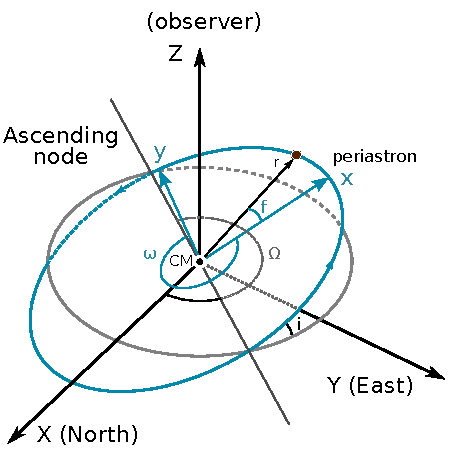
\includegraphics{orbit3D.pdf}
  \figcaption{A 3D representation of the orbit of the secondary star around the center of mass (CM). In this representation, $\omega = \omega_2$, and the ascending node is where the secondary crosses the plane of the sky moving away from the observer. In order to represent the orbit of the primary star about the CM, all parameters remain the same except $\omega_1 = \omega_2 + \pi$.
  \label{fig:orbit3D}}
  \end{center}
\end{figure}

Several of the orbital parameters describing the primary star orbit (around the center of mass) and the secondary star orbit (around the center of mass) are identical, e.g., period $P$, eccentricity $e$, inclination $i$, and longitude of the ascending node $\Omega$. The parameters that are different, then, are the semi-major axis, velocity semi-amplitude, and argument of periastron. The semi-major axes of each ellipse about the center of mass are related by
\begin{equation}
  a_1 = \frac{M_2}{M_1 + M_2} a
\end{equation}
\begin{equation}
  a_2 = \frac{M_1}{M_1 + M_2} a
\end{equation}
where $a = a_1 + a_2$ and is the semi-major axis of the binary orbit. The semi-amplitudes ($K$) of the radial velocity orbit are given by
\begin{equation}
  q = \frac{K_1}{K_2} = \frac{M_1}{M_2}.
\end{equation}
Lastly, the argument of periastron for each orbit differs by $\pi$, i.e., $\omega_1 = \omega_2 + \pi$. As we are deriving the equations of motion, it is important to keep in mind that the primary and secondary orbits do not share all the same parameters. First, we derive the equations of motion for a generic orbit (using $\omega$), since these will be the same rotation equations for both the primary and secondary orbits. However, in the perifocal plane of either the primary or secondary orbit (i.e., the orbital plane $x$-$y$), the argument of periastron is always where the orbit crosses the positive $x$ axis. So, to translate these orbits to the sky frame ($X$,$Y$,$Z$), the arguments of periastron will differ by a factor of $\pi$, as previously noted. What follows is basically re-deriving the contents of \citet{murray10} while respecting the convention changes that we noted.

\section{Astrometric Positions}
The main task of deriving equations of motion for RV and astrometric analysis is rotating the orbit from the perifocal plane to its orientation on the sky. To do this, we consider the rotation matrices
\begin{equation}
  {\bf P}_x(\phi) = \left [
  \begin{array}{ccc}
    1 & 0 & 0 \\
    0 & \cos \phi & - \sin \phi \\
    0 & \sin \phi & \cos \phi \\
    \end{array}\right]
\end{equation}
\begin{equation}
  {\bm P}_z (\phi) = \left [
  \begin{array}{ccc}
    \cos \phi & - \sin \phi & 0\\
    \sin \phi & \cos \phi & 0 \\
    0 & 0 & 1 \\
    \end{array}\right].
\end{equation}
These rotation matrices result in a \emph{clockwise} rotation of the axes, as defined using the right hand rule. This means when we look down the $z$-axis, for a positive angle $\phi$, it would be as if the $x$ and $y$ axes rotated clockwise.
In order to find out what defines counter-clockwise when considering the other rotations, we look to the right hand rule and cross products of the axes unit vectors. Since, $\hat{\bm x} \times \hat{\bm y} = \hat{\bm z}$, we know that when looking down the $z$ axis the direction of the $x$-axis towards the $y$-axis defines counter clockwise.
Similarly, we have $\hat{{\bm y}} \times \hat{{\bm z}} = \hat{{\bm x}}$, and $\hat{{\bm z}} \times \hat{{\bm x}} = \hat{{\bm y}}$.

To follow a useful description from \citet{murray10}, one can see how we need to rotate by referencing Figure~\ref{fig:orbit3D}. The three rotations are (i) a rotation about the $z$-axis through an angle $\omega$ so that the $x$-axis coincides with the line of nodes at the ascending node (ii) a rotation about the $x$-axis through an angle ($-i$) so that the two planes are coincident and finally (iii) a rotation about the $z$-axis through an angle $\Omega$. As one might notice, we break from \citet{murray10} in using a negative rotation for inclination, which is due to the change in how we label the ascending node. Applying these rotation matrices yields
\begin{equation}
  \left [ \begin{array}{c}
  X \\
  Y \\
  Z \\
\end{array}
  \right ] =
  {\bm P}_z (\Omega) {\bm P}_x(-i) {\bm P}_z(\omega)
  \left [
  \begin{array}{c}
  x \\
  y \\
  z \\
  \end{array}
  \right]
\end{equation}
and
\begin{equation}
  \left [
  \begin{array}{c}
    x \\
    y \\
    z \\
  \end{array} \right ]
  =
  {\bm P}_z^{-1}(\omega) {\bm P}_x^{-1}(-i) {\bm P}_z^{-1}(\Omega)
  \left [
  \begin{array}{c}
    X \\
    Y \\
    Z \\
    \end{array}
  \right ]
\end{equation}
The inverse of a rotation matrix is simply its transpose. Using the identities $\cos(- \phi ) = \cos \phi$, $\sin(- \phi) = -\sin \phi$, and the sum angle identities to simplify the calculations, we find
\begin{equation}
  \begin{array}{lc}
    X =& r (\cos \Omega \cos(\omega + f) - \sin(\Omega) \sin(\omega + f) \cos(i)) \\
    Y =& r (\sin \Omega \cos(\omega + f) + \cos(\Omega) \sin(\omega + f) \cos(i)) \\
    Z =& - r \sin(\omega + f) \sin(i).\\
\end{array}
\label{eqn:Z}
\end{equation}
A little surprisingly, these are the exact same equations for $X$ and $Y$ as found in \citet{murray10}. Because we used a different convention for $\Omega$ (offset by a factor of $\pi$), this necessitated remeasuring $\omega$, which was also offset by $\pi$ as well. The change in labeling ascending node also necessitates a different sense of rotation for inclination, but since $\sin (\phi + \pi) = - \sin \phi$ and $\cos (\phi + \pi) = -\cos \phi$, and $X$ and $Y$ have terms with both in them, a $\pi$ difference for both $\Omega$ and $\omega$ at the same time would cancel out (since the change in inclination rotation has not affected $\cos(-i) = \cos i$).
Our equation for $Z$ is different from \citet{murray10} because it now has a negative sign out front (due to the change in rotation for $i$ because of how we measure $\omega$).

If we are going to use these equations for astrometry, then it is important to note how we use the radius between the stars. The quantity $r$ is simply the separation between the stars,
\begin{equation}
  r = \frac{a (1 - e^2)}{1 + e \cos f},
  \label{eqn:r}
\end{equation}
so it should never be negative.
%\footnote{It is confusing that \citet{murray10} use negative values for $r_2$ in their equations.} 
If we are going to measure relative to the center of mass, then we will want to use the radius from the center of mass to that star
\begin{equation}
  r_1 = \frac{M_2}{M_1 + M_2} r,
\end{equation}
\begin{equation}
  r_2 = \frac{M_1}{M_1 + M_2} r.
  \label{eqn:r2}
\end{equation}
To find the astrometric positions for either star relative to the CM, we will use the formulae in Equation~\ref{eqn:Z} with the $\omega$ and radius appropriate for that star (e.g., ($\omega_1$, $r_1$) or ($\omega_2$, $r_2$)). If we wish to find the astrometric positions of the secondary star relative to the primary star (as measurements are commonly reported), then we would use the formulae in Equation~\ref{eqn:Z} with $\omega_2$ and the full value for $r$ (Equation~\ref{eqn:r}).

\subsection{Useful quantities}
For plotting purposes, it may be helpful to label things like periastron passage and the ascending node. The periastron is simply the point in the orbit where $f = 0$, so we have
\begin{equation}
  \begin{array}{lc}
    X =& r (\cos \Omega \cos(\omega) - \sin(\Omega) \sin(\omega) \cos(i)) \\
    Y =& r (\sin \Omega \cos(\omega) + \cos(\Omega) \sin(\omega) \cos(i)) \\
    Z =& - r \sin(\omega) \sin(i).\\
\end{array}
\end{equation}
The ascending node is where the secondary crosses the plane of the sky, moving away from the observer. So we set $Z = 0$ and solve
\begin{equation}
  Z = - r \sin(\omega + f ) \sin(i)
\end{equation}
beyond trivial solutions ($r = 0$, $i = 0$), the solution requires that $\omega + f = 0$ or $\omega + f = \pi$. Since the argument of periastron is measured from the ascending node in the direction of the orbital motion ($f$ increasing), then we know that the $\omega + f = 0$ solution must point to the ascending node. Therefore the true anomaly that yields the position of the ascending node is
\begin{equation}
  f_\Omega = -\omega = 2 \pi - \omega.
\end{equation}

\subsection{Polar Form}
While the formulae in Equation~\ref{eqn:Z} are useful for plotting 3D representations of the orbit, we often want to measure the separation ($\rho$) and position angle ($\theta$, measured East of North) of the secondary relative to the primary, as is commonly reported in the literature. In this case, we will utilize the equations for $X$ (North) and $Y$ (East) using $\omega_2$ and $r$.
\begin{equation}
  \rho = \sqrt{X^2 + Y^2}
\end{equation}
\begin{equation}
  \theta = \tan^{-1}\left (\frac{Y}{X} \right )
\end{equation}
where the inverse tangent operation should be carried out using a numerical library that respects the quadrants, e.g. \texttt{atan2(Y, X)}. To convert from polar coordinates to Cartesian coordinates in the sky plane, we would use
\begin{eqnarray}
  \Delta \delta =& X = \rho \cos \theta \\
  \Delta \alpha \cos \delta =& Y = \rho \sin \theta.
\end{eqnarray}

\section{Radial Velocities}
Next, we derive the radial velocity for our orbital conventions by finding the component of the velocity vectors of each star projected along the $Z$-axis
\begin{equation}
v_{Z,1} = \dot{{\bm r}}_1 \cdot \hat{{\bm Z}} = \frac{M_2}{M_1 + M_2} \dot{Z} 
\end{equation}
\begin{equation}
v_{Z,2} = \dot{{\bm r}}_2 \cdot \hat{{\bm Z}} = \frac{M_1}{M_1 + M_2} \dot{Z}
\end{equation}
where $\dot{Z}$ is measured using $r$, the separation between stars. We can derive $v_Z = \dot{Z}$ from Equation~\ref{eqn:Z} using the chain rule
\begin{equation}
  \dot{Z} = - \dot{r} \sin(\omega + f) \sin(i) - r \dot{f} \cos(\omega + f) \sin(i).
  \label{eqn:chain}
\end{equation}
If we define
\begin{equation}
  n = \frac{2 \pi}{P}
\end{equation}
and borrow two equations from \citet{murray10},
\begin{equation}
  \dot{r} = \frac{r \dot{f} \, e \sin f}{1 + e \cos f}
\end{equation}
and
\begin{equation}
  r \dot{f} = \frac{n a }{\sqrt{1 - e^2}} (1 + e \cos f),
\end{equation}
then we can rearrange Equation~\ref{eqn:chain} to
\begin{equation}
  \dot{Z} = -\frac{n a \sin i}{\sqrt{1 - e^2}} (\cos (\omega + f) + e \cos \omega).
\end{equation}
Here we introduce the semi-amplitudes
\begin{equation}
  K_1 = \frac{M_2}{M_1 + M_2} \frac{n a \sin i}{\sqrt{1 - e^2}}
\end{equation}
\begin{equation}
  K_2 = \frac{M_1}{M_1 + M_2} \frac{n a \sin i}{\sqrt{1 - e^2}}
\end{equation}
and find
\begin{eqnarray}
  v_{Z,1} =& - K_1 (\cos (\omega_1 + f) + e \cos \omega_1) \\
  v_{Z,2} =& - K_2 (\cos (\omega_2 + f) + e \cos \omega_2).
\end{eqnarray}
We are not quite done, since astronomers define a positive radial velocity as implying a redshifted source (moving away from us), and our $Z$-axis convention defines a positive $v_Z$ as moving towards the observer. Therefore, we need to flip the negative sign to be in agreement with radial velocity convention, i.e. $v_r = -v_Z$
\begin{eqnarray}
  v_{r,1} =& K_1 (\cos (\omega_1 + f) + e \cos \omega_1) \\
  v_{r,2} =& K_2 (\cos (\omega_2 + f) + e \cos \omega_2).
\end{eqnarray}

Happily, this is again consistent with the literature in general, including \citet{murray10}.\footnote{As drawn, \citet[Figure 7,][]{murray10} is inconsistent with these equations for radial velocity due to the aforementioned convention with $Z$ pointing towards the observer. If one assumes that $\omega = \omega_1$, then technically their Equation 65 should have a negative sign for $v_r$. After comparing equations, it seems as though it must be that in this equation $\omega = \omega_2$. An RV-only orbit is not sensitive to the value of $\Omega$, but a $\pi$ shift in $\omega$ will negate the radial velocities about the systemic velocity, thus delivering consistent equations of motion.} %I believe it is this sleight of hand that allows the whole framework to still yield consistent results, even though the conventions for $\Omega$ and $\omega$ were offset by factors of $\pi$.}
The end result of our analysis is that we find one can follow the derivations in \citet{murray10} to fit RV and astrometric data and still end up with correct equations for $X$, $Y$, and $v_r$ while also respecting the visual binary convention for labeling the ascending node. To compare our orbits to papers using the equations in \citet{murray10}, we need to add $\pi$ to $\Omega$ to convert from their definition of the ascending node (secondary coming towards us, what we call the descending node) to ours (secondary receding from us).

\subsection{Fitting individual systems with these conventions}
To confirm that we have derived consistent equations of motion, we reproduce several joint RV + astrometric fits in the literature. For papers that explicitly follow our conventions, we entirely reproduce their published results. For papers that use alternate conventions of the ascending node, we achieve consistent orbits after converting to our conventions.

\paragraph{$\Sigma$248} is fit by \citet{torres95}, and we are able to exactly reproduce their orbit using the stated values in the paper and treating $\omega = \omega_2 =172.6^\circ$ (confirmed via private communication).

\paragraph{HD 10009} is fit by \citet{pourbaix98}, and we are able to exactly reproduce their orbit using the stated values in the paper and treating $\omega = \omega_2 = 251.6^\circ$.

\paragraph{GJ 3305AB} is fit by \citet{montet15}. We are able to reproduce their orbits if we use $\omega = \omega_1 = -69^\circ$, and assume that $\Omega = 18.8^\circ$ points to the \emph{descending node}, so we would use $\Omega = 18.8^\circ + 180^\circ$. Montet was explicit that he uses the planetary science convention where $\Omega$ points to the node where the secondary is coming towards us (our descending node), so this explains the $\Omega$ flip (private communication).

\paragraph{Gl 570BC} is fit by \citet{forveille99}. We are able to reproduce their orbits if we use $\omega_1 = 127.56^\circ$ and treat their $\Omega_1$ as measuring the \emph{descending node}. So we use $\Omega = 195.9^\circ + 180^\circ$. This is somewhat surprising, since we expected these authors to follow the visual binary conventions rather than the planetary science conventions.

\paragraph{41 Dra} is fit by \citet{tokovinin03}. We are able to reproduce their orbits if we use $\omega_a = \omega_1 = 127.31^\circ$ and treat their $\Omega_a$ as measuring the \emph{descending node}, or, equivalently, the ascending node of the primary. So we use $\Omega = 1.9^\circ + 180^\circ$. Again, we are somewhat surprised by the choice of the planetary science conventions, but seems plausible since \citet{forveille99} used a similar code by Tokovinin to fit the orbits.\footnote{See \url{http://www.ctio.noao.edu/~atokovin/orbit/Instruction.txt} for confirmation of this assumption.}

\section{Deriving the angular momentum vector ${\bm h}$}
Now that we have defined equations for the stellar orbit, we would like to compare its orientation to that of other orbits in the system, for example a circumbinary disk. To do this, we need to calculate the angular momentum vectors of the stellar orbits and the disk. From \citet[Eqn 5,][]{murray10}, we have
\begin{equation}
  {\bm h} = r^2 \dot{\theta} \, \hat{\bm z} =  h \, \hat{\bm z}
\end{equation}
where
\begin{equation}
  h = \sqrt{G\,(M_1 + M_2)\, a \, (1 - e^2)}.
\end{equation}
In this case, we use $a = a_1 + a_2$, since we are talking about the total angular momentum of the orbit (not just a single star). Then, we rotate this angular momentum vector to the $X$, $Y$, $Z$ frame using the same rotation matrices as before, to yield
\begin{equation}
  {\bm h} = h(-\sin \Omega \sin i \, \hat{\bm X} + \cos \Omega \sin i \, \hat{\bm Y} + \cos i \, \hat{\bm Z}).
  \label{eqn:angular_mom}
\end{equation}

\subsection{Comparing to the orientation of a disk}

\paragraph{Relative orientation} To compare the orientation of the orbit to that of the circumbinary disk, first we need to represent the orientation of the disk using the same coordinate system. Traditionally \citep[e.g.,][]{czekala15a}, we follow the same inclination convention as the astrometric orbit, but use a slight modification for position angle. The disk convention uses the angle formed between North and the projection of the disk angular momentum vector onto the sky plane as the variable $\varphi$, measured East of North. Compared to the position angle of the ascending node (again, defined where material is receding from the observer, or going into the plane of the sky), the two are related by
\begin{equation}
  \Omega_\mathrm{d} = \varphi - \pi/2
\end{equation}
where the subscript d represents a quantity for the disk. Then, we can write ${\bm h}_\mathrm{d}$ using Equation~\ref{eqn:angular_mom} and find the angle it forms with stellar orbital angular momentum vector ${\bm h}_\mathrm{o}$ using the dot product formula
\begin{equation}
  \cos \Phi = \frac{{\bm h}_\mathrm{o} \cdot {\bm h}_\mathrm{d}}{|{\bm h}_\mathrm{o}| |{\bm h}_\mathrm{d}|}
\end{equation}
\begin{equation}
  \cos \Phi = \sin \Omega_\mathrm{d} \sin i_\mathrm{d} \sin \Omega_\mathrm{o} \sin i_\mathrm{o} + \cos \Omega_\mathrm{d} \sin i_\mathrm{d} \cos \Omega_\mathrm{o} \sin i_\mathrm{o} + \cos i_\mathrm{d} \cos i_\mathrm{o}.
\end{equation}

Using the cosine sum trigonometric identity, we arrive at the same equation as in \citet{fekel81}
\begin{equation}
  \cos \Phi =  \cos i_\mathrm{d} \cos i_\mathrm{o} + \sin i_\mathrm{d} \sin i_\mathrm{o} \cos (\Omega_\mathrm{d} - \Omega_\mathrm{o}).
\end{equation}

\paragraph{Relative orientation of binary eccentricity vector}


\paragraph{Absolute value of disk angular momentum}
To determine the magnitude of the angular momentum vector of the rotating protoplanetary disk ${\bm h}_\mathrm{d}$, we must integrate the surface density profile of the disk along the radial direction. The gas is assumed to orbit in the disk in circular Keplerian orbits, with only an azimuthal component of velocity that is a function of the central stellar mass, $M_\ast$
\begin{equation}
	v_\phi(r) = \sqrt{\frac{G M_\ast}{r}}.
\end{equation}
We assume that the standard \citet{lynden-bell74} similarity solution describes the surface density profile,
\begin{equation}
\Sigma(r) = \Sigma_c \left (\frac{r}{r_c} \right)^{- \gamma} \exp \left[ - \left(\frac{r}{r_c} \right)^{2 - \gamma} \right]
\end{equation}
 where the critical radius $r_c$ denotes the transition from a power law to exponential taper and the pre-factor $\Sigma_c$ normalizes the profile. 
The differential angular momentum in a segment of the disk is\footnote{dropping the `d' subscript for brevity.}
\begin{equation}
\mathrm{d}{\bm h} = {\bm r} \times \mathrm{d}m {\bm v} = {\bm r} \times {\bm v} \Sigma({\bm r}) \, \mathrm{d}A  
\end{equation}
Because the disk velocity is always in the $\hat{{\bm \phi}}$ direction, this means that ${\bm r} \times {\bm v} = rv_\phi(r) \hat{{\bm z}}$.
\begin{equation}
\mathrm{d}{\bm h} = {\bm r} \times {\bm v} \Sigma({\bm r}) \mathrm{d}A = r v_\phi(r) \Sigma(r) \, \mathrm{d}A \, \hat{{\bm z}}.
\end{equation}
We have
\begin{equation}
{\bm h} = \int_A \mathrm{d}{\bm h} = 2 \pi \int_{r_\mathrm{in}}^{r_\mathrm{out}} r v_\phi(r) \Sigma(r) \, r \mathrm{d}r \, \hat{{\bm z}}
\end{equation}
where we implicitly perform the integral over the $\phi$ coordinate. Substituting for $v_\phi$ and $\Sigma$, we have
\begin{equation}
{\bm h} =  2 \pi \Sigma_c \sqrt{G M_\ast} \int_{r_\mathrm{in}}^{r_\mathrm{out}} r^{3/2} \left (\frac{r}{r_c} \right)^{- \gamma} \exp \left[ - \left(\frac{r}{r_c} \right)^{2 - \gamma} \right] \, \mathrm{d}r \, \hat{{\bm z}}.
\end{equation}
This integral can be performed numerically.
The total disk mass ($M_\mathrm{disk}$) can be found by integrating $\Sigma(r)$ over the surface area of the disk. 


\vspace{5mm}

\acknowledgements
I.C. would like to thank Guillermo Torres, Eric Nielsen, and Ben Montet for extensive help and conversations when discussing orbits and orbital conventions.

\bibliographystyle{aasjournal.bst}
\bibliography{orbit.bib}

\end{document}
